\section{Evaluation\label{sec:evaluation}}
TimeTubesX is a browser-based application written in HTML and Javascript.
We use React.js to build user interfaces and flux.js to manage the application states.
We also utilize standard libraries such as three.js~\cite{three_framework}, D3.js~\cite{d3_framework}, and Paper.js~\cite{paper_framework}.
TimeTubesX is open-source (\url{https://github.com/MistletoeNaoko/TimeTubesWeb}), and 
% the running system can be found at \url{https://timetubes.herokuapp.com/}.
readers can try the running system with our synthetic data at \url{https://timetubes.herokuapp.com/}.

We shared TimeTubesX with four domain experts, three of whom we interviewed for the domain analysis in Section 3.2: the second author of this paper (astronomer 1), astronomer 1’s former master course student (astronomer 2), an assistant professor at Hiroshima University (astronomer 3), and a postdoc at Stanford University (astronomer 4). Sections \ref{sec:correlate} and \ref{sec:anticorrelate} present two case studies by astronomer 1 and Section \ref{sec:whatif} discusses the cause of the phenomena presented in Section \ref{sec:anticorrelate}. Section \ref{sec:feedback} introduces qualitative feedback from the four domain experts.
% In this section, we present and discuss two real-world data analysis sessions and feedback from two domain experts at Hiroshima University, who are a co-author of this paper and his former master course student, respectively.
% In this section, first, we present and discuss two real-world data analysis sessions using the blazar datasets described in~\cite{Gaur2014} that were performed by a domain expert at Hiroshima University, who is a co-author of this paper.
% And then, we report feedback from two domain experts, 
% who are the co-author and a  at Hiroshima University.
To examine the magnetic field structures in the jets, 
astronomers analyze polarimetric observations. 
Through the analysis of correlations between polarization and intensity, 
they validate multiple hypotheses for the increase in the intensity ($I$). 
The two case studies were performed by astronomer 1, using the datasets for the blazar \emph{BL Lac}. 
It was previously empirically noted in \cite{Gaur2014} that $I$ of \emph{BL Lac} tends to anti-correlate with the polarization degree ($PD$) during a certain period.
% It was previously empirically noted in \cite{Gaur2014} that the intensity ($I$) of \emph{BL Lac} tends to anti-correlate with the polarization degree ($PD$) during a certain period.
% The observation datasets for \emph{BL Lac} include 285 observations over a period of about 3.5 years.
On a MacBook Pro 2017 with a 3.5 GHz Intel Core i7 and a 16 GB RAM, it took 1{,}193 ms and 1{,}236 ms to obtain the results mentioned in Section~\ref{sec:correlate} and Section~\ref{sec:anticorrelate}, respectively.
%

% \subsection{Implementation and performance}
% TimeTubesX is a browser-based application written in HTML and Javascript.
% We use React.js to build user interfaces and flux.js to manage the application state.
% We also utilize standard libraries such as D3.js~\cite{d3_framework} and paper.js~\cite{paper_framework}.
% TimeTubesX is open-source and running system can be found at \url{https://timetubes.herokuapp.com/}.

% On a MacBook Pro 2017 with a 3.5 GHz Intel Core i7 and 16 GB RAM, it took 1{,}193 ms and 1{,}236 ms to get the results mentioned in \autoref{sec:correlate} and \autoref{sec:anticorrelate}, respectively.
% removed: , an Intel Iris Plus Graphics 650 1536 MB

% \subsection{Correlation analysis of $I$ and $PD$}\label{sec:correlate}
\subsection{Case Study 1: Correlation Patterns of $I$ and $PD$}\label{sec:correlate}
\begin{figure}[tb]
    \centering
    \begin{minipage}{0.49\linewidth}
        \centering
        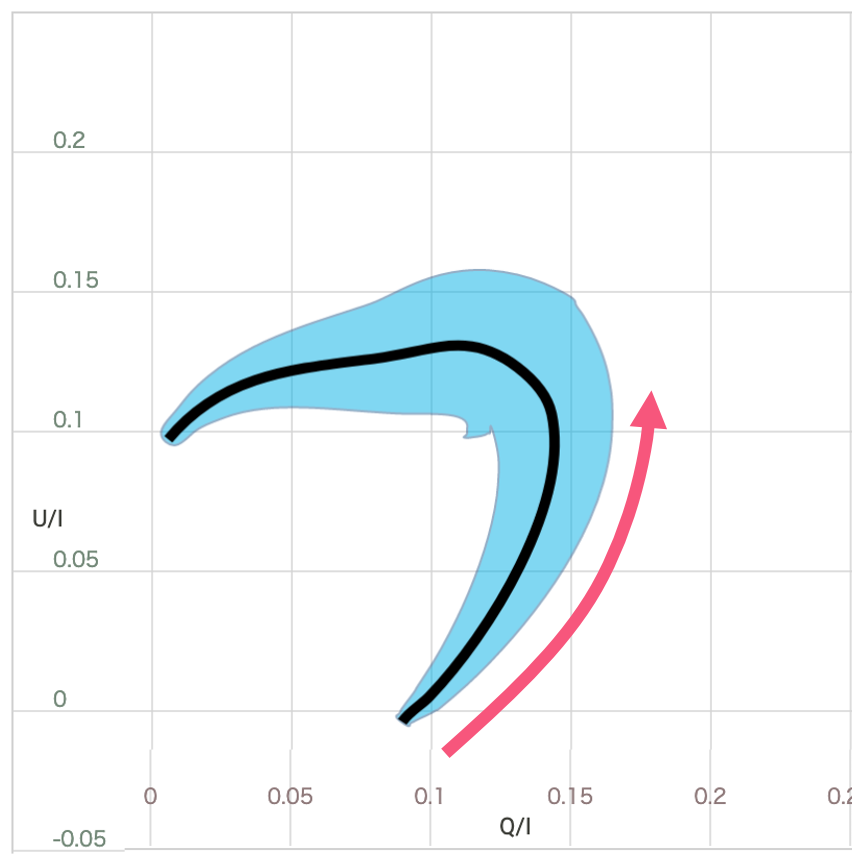
\includegraphics[width=.9\linewidth]{vgtc_journal_latex/figures/QBScorrelate.png}\\
        \footnotesize{\sf(a)~A query for a correlated $I$ and $PD$ variation.}\\
    \end{minipage}
    \begin{minipage}{0.49\linewidth}
        \centering
        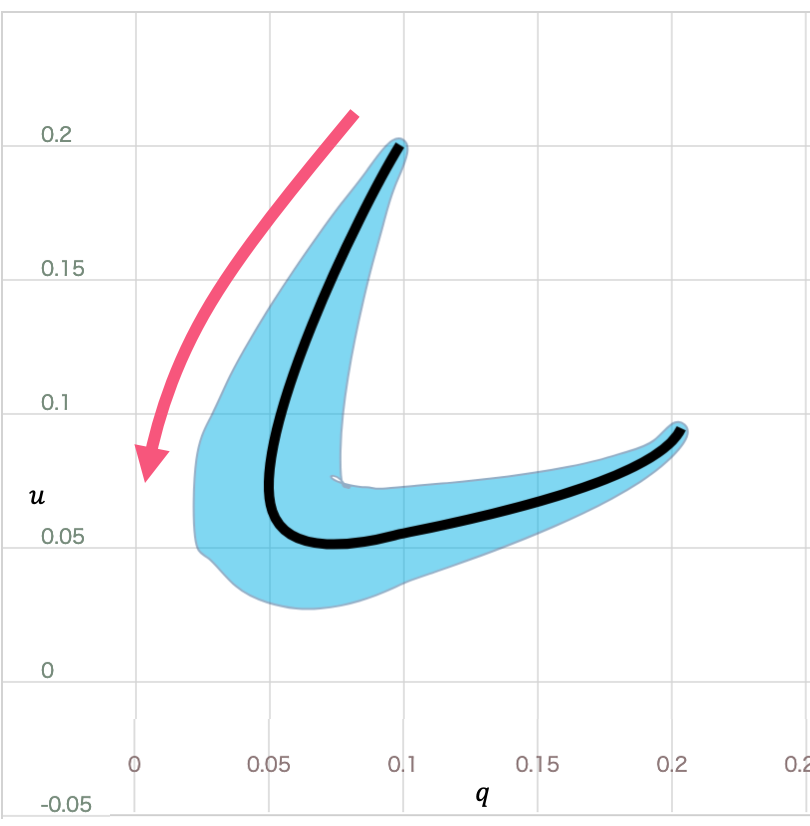
\includegraphics[width=.9\linewidth]{vgtc_journal_latex/figures/QBSanticorrelate.png}\\
        \footnotesize{\sf(b)~A query for an anti-correlated $I$ and $PD$ variation.}\\
    \end{minipage}
    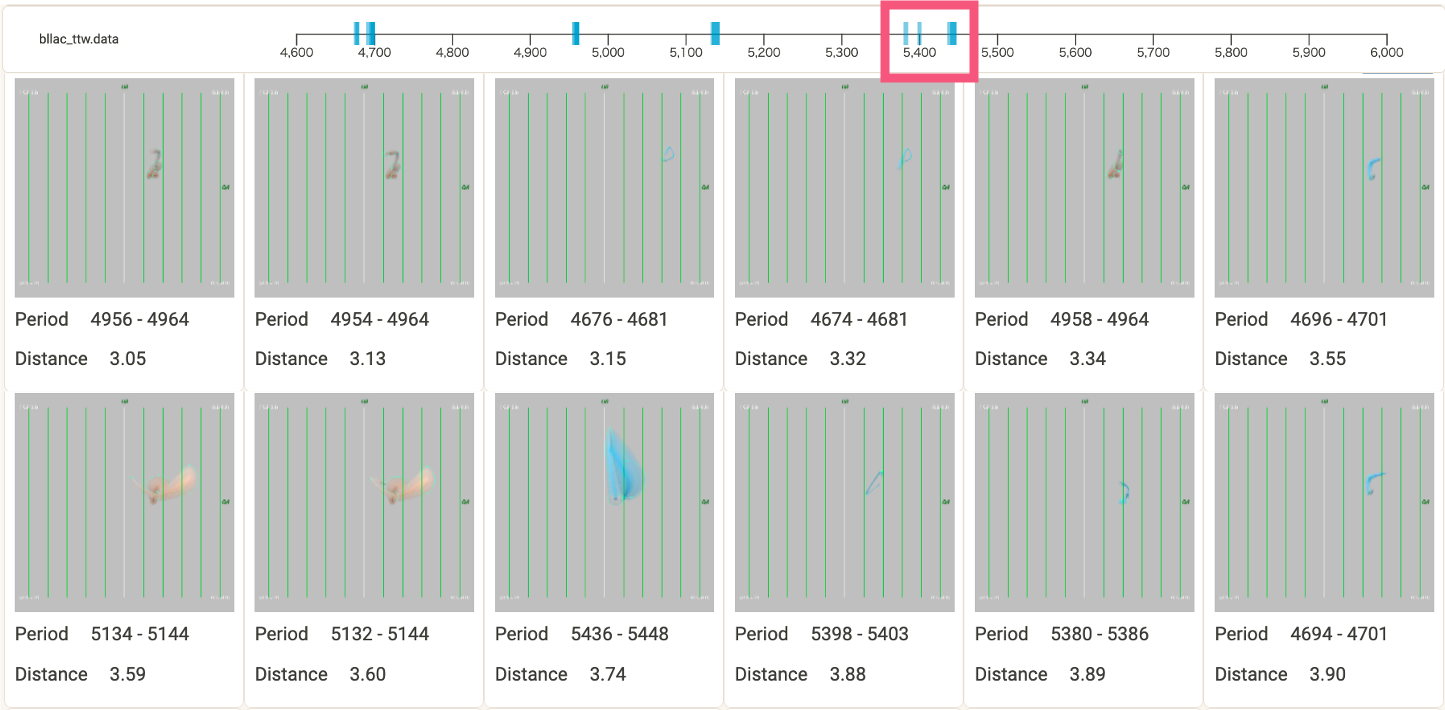
\includegraphics[width=.99\linewidth]{vgtc_journal_latex/figures/correlateResultsLabel14.png}\\
    \footnotesize{\sf(c)~Top 12 time intervals similar to the query in (a).}\\
    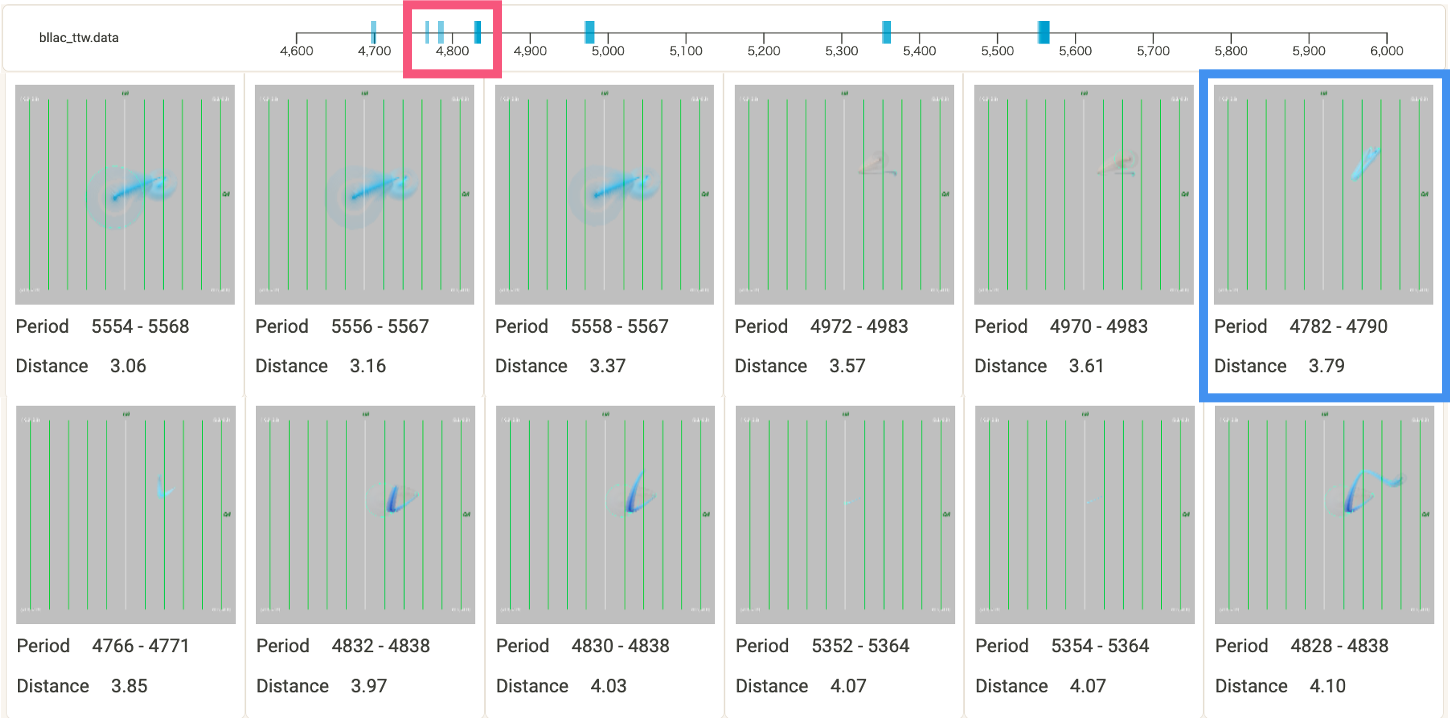
\includegraphics[width=.99\linewidth]{vgtc_journal_latex/figures/anticorrelateResultsLabel14.png}\\
    \footnotesize{\sf(d)~Top 12 time intervals similar to the query in (b).}
    \caption{Analysis of the blazar \emph{BL Lac} to investigate correlation patterns between $I$ and $PD$. (a) and (b) are user-drawn sketches. (c) and (d) are the results of QBS with the queries shown in (a) and (b), respectively.}
    \label{fig:EvaluationQueryResults}
\end{figure}
%
Astronomer 1's goal in these case studies was to identify global statistical features of the period of interest and to build a hypothesis of correlations between the time variations of $I$ and $PD$.
To achieve this goal, he had to meticulously analyze correlations between $I$ and $PD$ in the entire time period and many short time intervals within that period.
However, it seemed difficult to manually take a close look at each of the short time intervals.
% analyze many short time intervals one by one.
Therefore, he decided to utilize QBS to investigate correlation patterns in a long-term observation dataset.

First, he built a hypothesis that an increase in $I$ tends to correlate with an increase in $PD$ in \emph{BL Lac}.
To validate this hypothesis and examine how frequently such behavior appears, he sketched the query shown in Fig.~\ref{fig:EvaluationQueryResults}~(a), 
%He started the sketch from the right edge and ended at the left edge.
where the $x$ and $y$ axes express $q$ and $u$, respectively, 
and the stroke width represents $I$.
Therefore, the input sketch indicates a pattern 
that $I$ gradually increases and then decreases, correlated to $PD$, which implies the distance from the origin of the Stokes plane.
To extract time intervals with a similar shape but different position or different scale, he used the normalization and polar coordinates options. 
To avoid missing short events, he set the warping window size and the sliding window size to 0 and 2, respectively.

Fig.~\ref{fig:EvaluationQueryResults}~(c) shows the top twelve results of the query sketched in (a).
The timeline at the top of (c) illustrates 
that the extracted time intervals seem to be distributed over the entire dataset.
However, in the period from $[5{,}350, 5{,}450]$ (enclosed by a red rectangle in (c)), 
the input pattern seems to occur more frequently than in other periods.
Visiting all time intervals in this period individually and analyzing them in the TimeTubes view,
some of them include the correlation pattern in (a),
but others do not.
Thus, he concluded that the input correlation pattern does not frequently occur in that period.
The reason for this misclassification could be that our system, due to the normalization option, detects time intervals with a relatively small variation of $I$ as well.
However, he was still highly pleased with TimeTubesX, as it allowed him to quickly identify a relatively small number of time intervals that he could then examine in more detail.
%Though such misclassifications can be included, 
%QBS could concentrate more on an enough smaller number of time intervals for him to visit them one by one.

%
\subsection{Case Study 2: Anti-Correlation Patterns of $I$ and $PD$}\label{sec:anticorrelate}
Astronomer 1 also noticed that the variation in $I$ tends to \emph{anti}-correlate with that in $PD$. %in \textbf{BL Lac}.
To detect time intervals with such anti-correlated $I$ and $PD$ patterns, he drew another query (Fig.~\ref{fig:EvaluationQueryResults}~(b)),
where the plane represents the Stokes plane and the stroke width $I$.
The sketch describes a pattern that $I$ gradually increases and then decreases, while $PD$ shows a negative correlation. %of first increasing and then decreasing.
%showing an inverse correlation with $PD$.
%gradually increases and then decreases while PD with a negative correlation of $PD$.
% For this query, 
He used the same matching parameters as in Section~\ref{sec:correlate}.

Fig.~\ref{fig:EvaluationQueryResults}~(d) shows the top twelve results of the query shown in (b).
Like the previous case study, 
extracted time intervals seem to be distributed over the entire dataset. % as shown on the timeline at the top of (d).
However, in the period from $[4{,}750, 4{,}850]$ (enclosed by a red rectangle in (d)), 
the input pattern seems to occur more frequently.
% The previous report by his group~\cite{Gaur2014}
His group previously reported that, statistically, the variation in $I$ anti-correlates with that in $PD$ during the years 2008 to 2010 in \emph{BL Lac}~\cite{Gaur2014}.
However, even in that previous report, they did not analyze short time intervals in the period individually.
By analyzing the extracted time intervals in the period with TimeTubesX, he could verify not only that an increase in $I$ globally tends to co-occur with a decrease in $PD$, 
but also that local peaks of $I$ are correlated with decreases in $PD$.

% These analysis examples
These case studies with QBS underline the importance of local analysis of short time intervals within a larger time period as well as a global analysis of the entire period.

%
%
\subsection{What-If Scenario Analysis}\label{sec:whatif}
This section explains how astronomers can identify what generally contributes to the $PD$ variation of blazars in a certain time period. 
% Furthermore, we outline how our domain expert could test a hypothesis like the example of negative correlation between $I$ and $PD$ mentioned in Section~\ref{sec:anticorrelate}.

Astronomers expect that $PD$ variation of a blazar is caused by either of the two following hypotheses:
\begin{enumerate}[nosep, label=\textsl{Hypothesis \arabic*}, align=parleft, leftmargin=*]
    \item \textsl{$total\,flux$ increases (decreases) due to the increase (decrease) in $unpolarized\,flux$}; or  \label{scenario1}
    \item \textsl{There are two polarized components, and they are perpendicular to each other}. \label{scenario2}
\end{enumerate}
Note that $PD$ can be derived from the amount of $flux$: $PD = \frac{polarized\,flux}{total\,flux}$,
where $total flux = I = polarized\,flux + unpolarized\,flux$.
Astronomers can identify which of the above hypotheses contributes to the decrease in $PD$
by comparing time variations of data samples of the time interval in the $q - u$ domain and in the $Q-U$ domain,
where $q = Q / I$ and $u = U / I$, as explained in Section~\ref{sec:BlazarData}.
In the case of \ref{scenario1}, the position of a data sample in the $q - u$ domain gradually moves toward the origin ($(q, u) = (0, 0)$),
whereas the position in the $Q-U$ domain does not move toward the origin ($(Q, U) = (0, 0)$),
because only the amount of $total flux$ increases.
On the other hand, in the case of \ref{scenario2}, 
$PD$ decreases due to a flare of another polarized component with $PA$ perpendicular to the jet direction.
The position of a data sample moves toward the origin both in the $q - u$ domain and in the $Q - U$ domain 
% because $Q$ and $U$ are denumerable values; 
because another polarized component influences observed $Q$ and $U$ values, 
implying that $q$ and $u$ (fractional values of $Q$ and $U$) are also influenced.
% specifically, when two polarized components perpendicular to each other exist, 
% the total $Q(t)$ and $U(t)$ of the two polarization sources at time $t$ are computed by $Q(t) = Q_1(t) + Q_2(t)$ and $U(t) = U_1(t) + U_2(t)$.
By comparing datasets for $(q, u)$ and $(Q, U)$ with the side-by-side option of the visual data fusion~\cite{Fujishiro2018},
plausibility of these hypotheses can be visually examined.
\begin{figure}[tb]
    \centering
    \includegraphics[width=.8\linewidth]{vgtc_journal_latex/figures/stokesComparisonLabel.png}
    % \begin{minipage}{.49\linewidth}
    %     \centering
    %     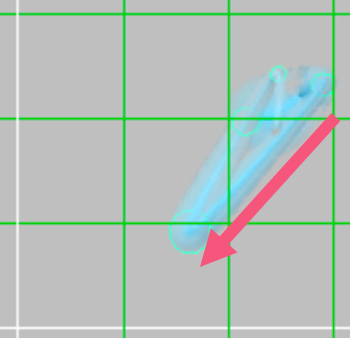
\includegraphics[width=.9\linewidth]{vgtc_journal_latex/figures/stokesComparisonLabelQIUI.png}\\
    %     \footnotesize{\sf(a)~$q - u$ domain.}
    % \end{minipage}
    % \begin{minipage}{.49\linewidth}
    %     \centering
    %     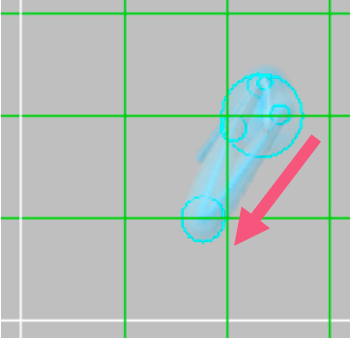
\includegraphics[width=.9\linewidth]{vgtc_journal_latex/figures/stokesComparisonLabelQU.png}\\
    %     \footnotesize{\sf(b)~$Q - U$ domain.}
    % \end{minipage}
    \caption{Comparison of a dataset consisting of $q$ and $u$ (left) and one consisting of $Q$ and $U$ (right) for the time interval $[4{,}782, 4{,}890]$.
    In both images, the position of a data sample goes toward the origin of the domain (lower left), which means this polarization variation was caused by the decrease in PD of a different polarized component.}
    \label{fig:comparisonQIUIvsQU}
\end{figure}

The following discussion considers the anti-correlation patterns of $I$ and $PD$, as mentioned in Section~\ref{sec:anticorrelate}.
Astronomer 1 did indeed compare a dataset consisting of $q$ and $u$ and one consisting of $Q$ and $U$. The comparison results at the time interval with a blue rectangle in Fig.~\ref{fig:EvaluationQueryResults}~(d) are shown in Fig.~\ref{fig:comparisonQIUIvsQU}.
As the red arrows in Fig.~\ref{fig:comparisonQIUIvsQU} indicate, 
he found that both data samples move toward the origin.
% , in the $q-u$ domain as well as in the $Q-U$ domain.
He found this behavior for all short time intervals in the period $[4{,}750, 4{,}850]$.
Thus, he finally concluded that the negative correlation of $I$ and $PD$ in the period is not due to the increase in $unpolarized flux$ (\ref{scenario1}) but due to the presence of two polarized components (\ref{scenario2}). 
% the decrease in $PD$ of a different polarized component (\ref{scenario2}). 

Overall, TimeTubesX greatly facilitated the detailed visual exploration of blazar data. This allowed the domain expert to examine many small time intervals with specific features, which was too laborious with previous methods.
%, allowing him to examine time intervals with a specific feature
%and contributes to more detailed analysis which was too laborious with the conventional methods.

% To avoid such misclassifications in general, users have to visit each detected time interval 
% and verify whether it satisfies their intentions with the line charts comparing the query and the time interval or TimeTubes view.

\subsection{Qualitative Feedback from Domain Experts}\label{sec:feedback}
Astronomer 2 found that the rotation detection was useful. 
With our rotation detection functionality, 
he was able to find three unknown rotation behaviors with shifted rotation center in the blazar \emph{3C 454.3}~\cite{Huang2019}. 
Astronomer 1, 3, and 4 mentioned that the QBS method was especially useful and helpful for validating their high-level hypotheses, as demonstrated in Sections~\ref{sec:correlate} and \ref{sec:anticorrelate}. Specifically, astronomer 3 and 4 said that the dynamic visual querying could be a powerful tool to examine jet physical processes and behaviors of plasma and magnetic fields under extreme conditions, because the dynamic visual querying can efficiently address arbitrary time variation patterns of polarization, intensity, and color. Astronomer 1 and 3 noticed TimeTubesX’s possibility for data mining. In particular, astronomer 3 saw massive potential for mining existing and upcoming large polarization surveys, while astronomer 1 found that a usage of TimeTubesX enables astronomers to identify interesting features in short time intervals, which cannot be achieved with conventional methods due to too many short time intervals in a long-term dataset. Furthermore, fact-guided querying was impressive for him because it allowed astronomers to refine their sketches based on actual extracted patterns.

% In addition to the case studies (Sections~\ref{sec:correlate} and \ref{sec:anticorrelate}),
% our domain experts were able to find three rotation behaviors in the blazar \emph{3C 454.3} that had not yet been described in the literature. 
% Whenever there are multiple polarization components in the same observation area, rotations cannot be identified just by analyzing $PA$ variations.
% They mentioned that identifying these patterns was only possible because TimeTubesX allowed them to analyze rotations whose centers are not at the origin of the Stokes plane~\cite{Huang2019}. 
% % The domain experts confirmed the usefulness of TimeTubesX. 
% They also found the visual queries helpful and impressive. 
% They mentioned that the QBS method was especially useful for validating their abstract hypotheses, as demonstrated in Sections~\ref{sec:correlate} and \ref{sec:anticorrelate}.
% According to them, TimeTubesX allowed them to identify interesting features in short time intervals.
% This cannot be achieved with conventional methods because there are too many short time intervals in a long-term dataset.
% Furthermore, fact-guided querying was crucial for them because it allowed them to refine their sketches based on actual extracted patterns.